\documentclass{standalone}
%% Show/hide steps for standalone work — edit this line:
\makeatletter\AtBeginDocument{\@buildstepset{1,2,2.5,3,4,4.5,5,6,7,8,9,10}}\makeatother
\usepackage{tikz}
\usetikzlibrary{intersections,calc}
\usepackage{amsmath}
\usepackage{hsbcommon}
\begin{document}
    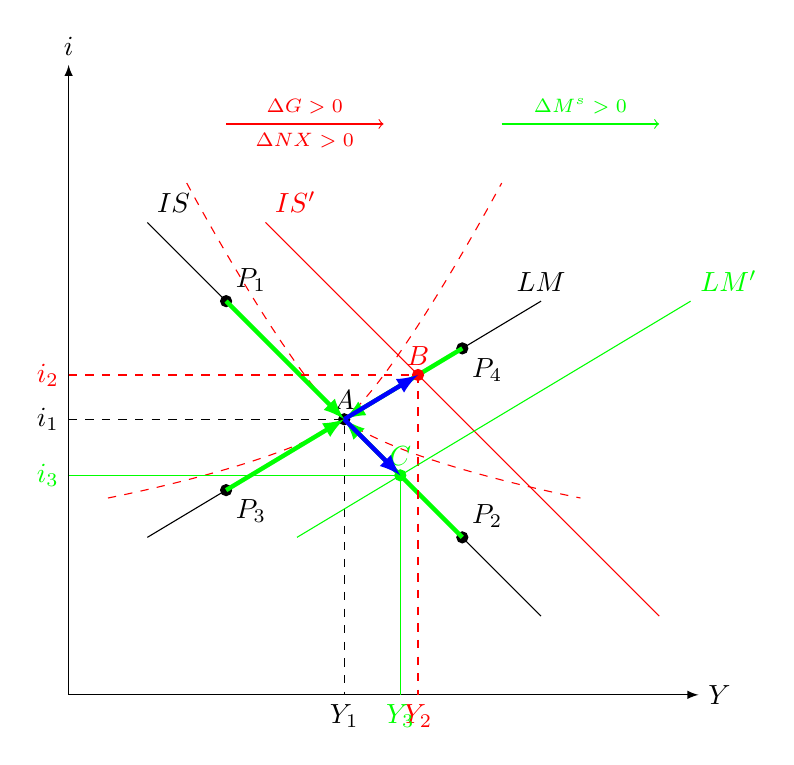
\begin{tikzpicture}
        \draw[->,>=latex] (0,0) -- (8,0) node (Y) [right] {$Y$};
        \draw[->,>=latex] (0,0) -- (0,8) node (i) [above] {$i$};

        \node[left] at (0,0) {\phantom{$i_1$}};

        \coordinate (A) at (1,6);
            % \coordinate (A2) at (2,2);
        \coordinate (B) at (6,1);
        
        \coordinate (C) at (1,2);
            % \coordinate (C2) at (5,2);
        \coordinate (D) at (6,5);
        \path[name path=is] (A) -- (B);
        \path[name path=lm] (C) -- (D);
        % \path[name path=is] plot[smooth] coordinates {(A) (A2) (B)};
        % \path[name path=lm] plot[smooth] coordinates {(C) (C2) (D)};
        \path [name intersections={of=is and lm, by=E}];

        %% some points out of equilibrium
            \coordinate (imbal3) at ($(C)!0.2!(D)$);
            \coordinate (imbal4) at ($(D)!0.2!(C)$);
            \coordinate (imbal1) at ($(A)!0.2!(B)$);
            \coordinate (imbal2) at ($(B)!0.2!(A)$);            

        %%  IS Curve
        \ifstep{1}{
            \draw[name path=is] (A) node[above right] {$IS$} -- (B);
        }


        %%  Points on IS

        \ifstep{2}{

            \filldraw (imbal1) node[above right] {$P_1$} circle (2pt);
            \filldraw (imbal2) node[above right] {$P_2$} circle (2pt);

        
        }

        \ifstep{2.5}{
            \draw[red,dashed] plot[smooth] coordinates {($(E)+(-2,3)$) (E) ($(E)+(3,-1)$)};    
        }



        %% LM Curve, equilibrium
        \ifstep{3}{
            \draw[name path=lm] (C) -- (D) node[above] {$LM$};

        }

        %% Points on LM
        \ifstep{4}{

            \filldraw (imbal3) node[below right] {$P_3$} circle (2pt);
            \filldraw (imbal4) node[below right] {$P_4$} circle (2pt);

        }

        \ifstep{4.5}{
            \draw[red,dashed] plot[smooth] coordinates {($(E)+(-3,-1)$) (E) ($(E)+(2,3)$)};    
        }

        %% Equilibrium

        \ifstep{5}{
            \filldraw (E) circle (2pt) node[above] {$A$};
            \draw[dashed] (i |- E) node [left] {$i_1$} -- (E) -- (E |- Y) node [below] {$Y_1$};        
        }


        \ifstep{2}{
            \ifstep{4}{
                \begin{scope}[red]

                    \draw[->,>=latex,green,ultra thick] (imbal1) -- (E);
                    \draw[->,>=latex,green,ultra thick] (imbal2) -- (E);
                    \draw[->,>=latex,green,ultra thick] (imbal3) -- (E);
                    \draw[->,>=latex,green,ultra thick] (imbal4) -- (E);
                    
                \end{scope}
            }
        }
        
        %% IS curve shift
        \ifstep{6}{
            \begin{scope}[color=red]
                    \draw[name path=is2] ($(A)+(1.5,0)$)   node[above right] {$IS'$} -- ($(B)+(1.5,0)$)  ;
                    \path [name intersections={of=is2 and lm, by=F1}];
                    \filldraw (F1) circle (2pt) node[above] {$B$};
                \draw[dashed] (i |- F1) node [left] {$i_2$} -- (F1) -- (F1 |- Y) node [below] {$Y_2$};
                \draw[->,>=latex,ultra thick, blue] (E) -- (F1);
                \draw[->] (2,7.25) -- node[above] {\scriptsize $\Delta G>0$} node[below] {\scriptsize $\Delta NX>0$} (4,7.25) ;

            \end{scope}
        }

        %% LM curve shift
        \ifstep{7}{
            \begin{scope}[color=green]
                % \draw [->] (6.7,6) -- node[above] {\scriptsize $\Delta M>0$} (7.5,6);
                \begin{scope}[xshift=1.7cm]
                    \draw[name path=lm2] ($(C)+(1.9,0)$)  -- ($(D)+(1.9,0)$)  node[above right] {$LM'$};
                    \path [name intersections={of=is and lm2, by=F2}];
                    \filldraw (F2) circle (2pt) node[above] {$C$};
                \end{scope}
                \draw (F2) -- (i |- F2) node [left] {$i_3$};
                \draw (F2) -- (F2 |- Y) node [below] {$Y_3$};
                \draw[->,>=latex,ultra thick, blue] (E) -- (F2);
                \draw[->] (5.5,7.25) -- node[above] {\scriptsize $\Delta M^s>0$} (7.5,7.25) ;

            \end{scope}
        }

    \end{tikzpicture}
\end{document}